%!TEX root = ../novoIndex.tex

Considerando a estratégia descrita na solução proposta, os resultados da execução das CNNs aplicadas ao problema de estimação de idade a partir de uma imagem de face são apresentados a seguir. Estes resultados estão organizados segundo abordagens sequenciais, que contemplam desde as técnicas mais elementares, e que vão aumentando o grau de complexidade conforme uso de estratégias específicas da prática de DL para a resolução de problemas práticos.

\section{Abordagem 1: LeNet e AlexNet com Imagens Normalizadas}%sem data augmentation, com normalização e sem equalização

	A primeira abordagem de treinamento considerou o uso dos modelos de maneira canônica, isto é, tais como são definidos na literatura. Adotou-se as funções de ativação não-lineares \emph{ReLU} e \emph{Leaky ReLU} por serem simples de calcular e por satisfazerem os critérios de continuidade e diferenciação, requeridos pelo algoritmo de \emph{backpropagation}, conforme discutido anteriormente na Seção \ref{subsec:modelos}.

	As imagens da base de dados foram normalizadas antes de serem apresentadas às redes. Todos os valores dos pixels componentes das imagens foram escalonados para o intervalo $[0,1]$ por meio de uma divisão por $255$. A prévia normalização das imagens antes da apresentação às CNNs colabora para uma melhor execução do gradiente descendente e diminui a variância nos pesos.

	Os treinamentos destas duas arquiteturas duraram aproximadamente $16$ e $12$ horas respectivamente, em uma instância do Google Compute Engine com 4 CPus virtuais e 15 GB de RAM. Os gráficos de treinamento e as retas zero obtidas a partir da apresentação do conjunto de teste aos modelos consolidados podem ser vistos na Figura \ref{fig:lenet-abordagem1}. É possível notar que ambas as redes sofreram \emph{overfitting} e obtiveram grande margem de erro.


	\begin{figure}[hb!]
		\caption{Resultados do treinamento e teste da CNN LeNet.}\label{fig:lenet-abordagem1}
	  \begin{subfigure}[hb]{0.5\linewidth}
	    \caption{RMSE de treinamento da arquitetura LeNet utilizando funções de ativação \emph{ReLU}.}
	    \label{fig:redeneuralbiologica}
	    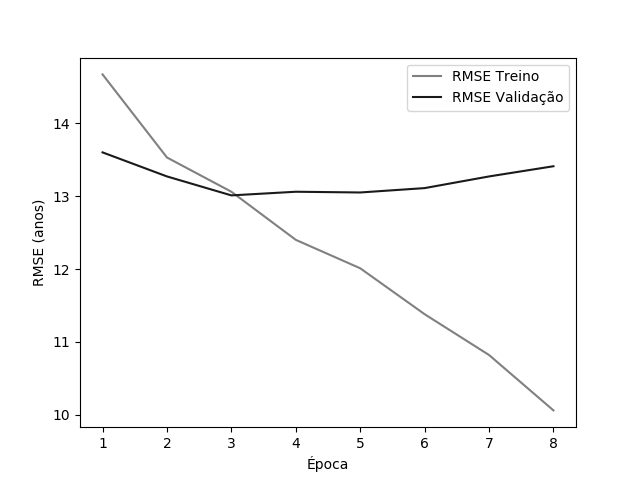
\includegraphics[width=\linewidth]{img/graficos/history/lenet/fig-history-image-treat-1-lenet-relu-rmse.png}%
	  \end{subfigure}%
		\begin{subfigure}[hb]{0.5\linewidth}
			\caption{Reta-0 LeNet \emph{ReLU}.}
			\label{fig:redeneuralbiologica}
			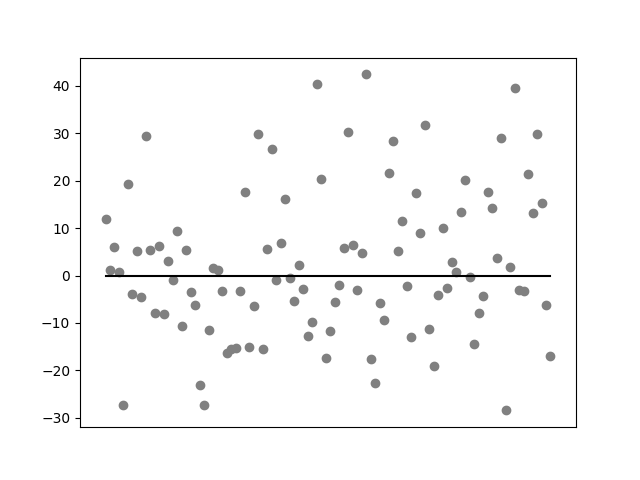
\includegraphics[width=\linewidth]{img/graficos/reta0/lenet/fig-reta-0-image-treat-1-lenet-relu.png}%
		\end{subfigure}\\
	  \begin{subfigure}[hb]{0.5\linewidth}
	    \caption{RMSE de treinamento da arquitetura LeNet utilizando funções de ativação \emph{Leaky ReLU}.}
	    \label{fig:redeneuralbiologica}
	    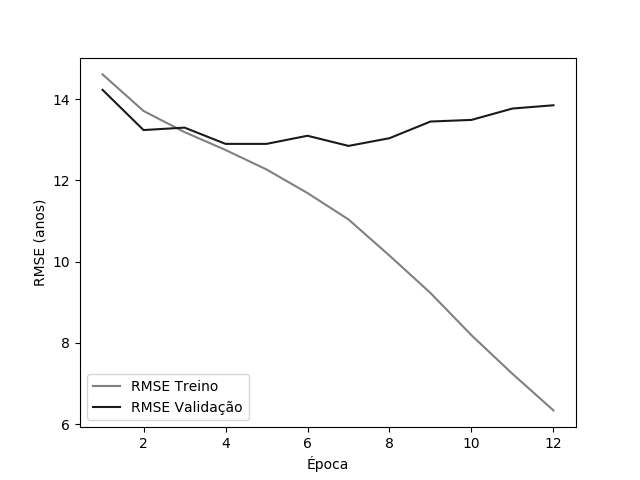
\includegraphics[width=\linewidth]{img/graficos/history/lenet/fig-history-image-treat-1-lenet-lrelu-rmse.png}
	  \end{subfigure}
		\begin{subfigure}[hb]{0.5\linewidth}
			\caption{Reta-0 LeNet \emph{Leaky ReLU}.}
			\label{fig:redeneuralbiologica}
		 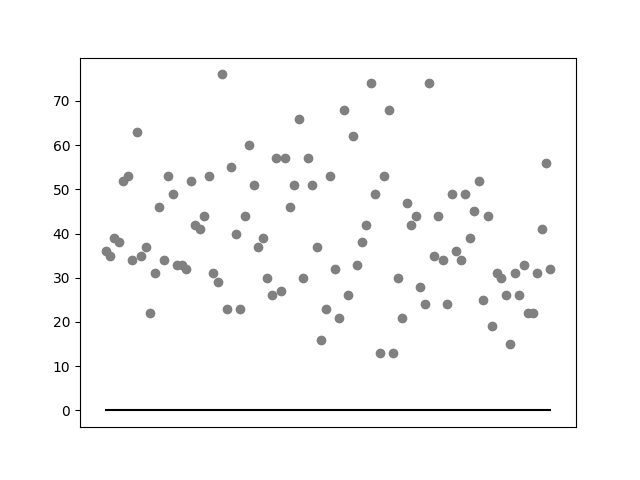
\includegraphics[width=\linewidth]{img/graficos/reta0/lenet/fig-reta-0-image-treat-1-lenet-lrelu.png}
		\end{subfigure}%
	\end{figure}

	\begin{figure}[hb!]
		\caption{Resultados do treinamento e teste da CNN AlexNet.}\label{fig:alexnet-abordagem1}
		\begin{subfigure}[hb]{0.5\linewidth}
			\caption{Treinamento AlexNet \emph{ReLU}.}
			\label{fig:redeneuralbiologica}
			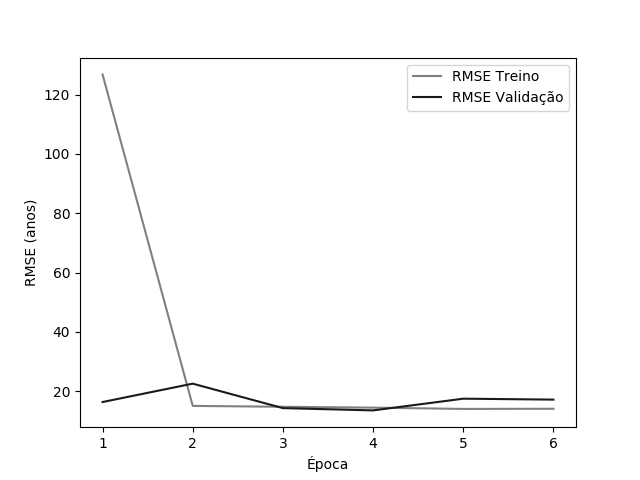
\includegraphics[width=\linewidth]{img/graficos/history/alexnet/fig-history-image-treat-1-alexnet-relu-rmse.png}
		\end{subfigure}
	  \begin{subfigure}[hb]{0.5\linewidth}
	    \caption{Reta-0 AlexNet \emph{ReLU}.}
	    \label{fig:reta0reludying}
	    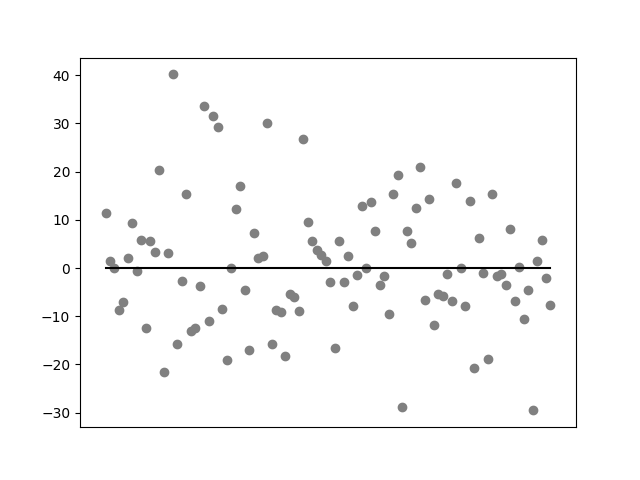
\includegraphics[width=\linewidth]{img/graficos/reta0/alexnet/fig-reta-0-image-treat-1-alexnet-relu.png}%
	  \end{subfigure}\\
		\begin{subfigure}[hb]{0.5\linewidth}
			\caption{Treinamento AlexNet \emph{Leaky ReLU}.}
			\label{fig:histalexlrelunorm}
	    \centering
			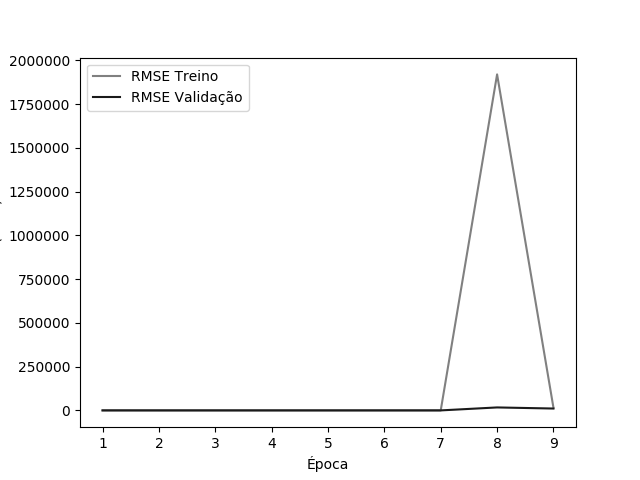
\includegraphics[width=\linewidth]{img/graficos/history/alexnet/fig-history-image-treat-1-alexnet-lrelu-rmse.png}
		\end{subfigure}
	  \begin{subfigure}[hb]{0.5\linewidth}
	    \caption{Reta-0 AlexNet \emph{Leaky ReLU}.}
	    \label{fig:redeneuralbiologica}
	    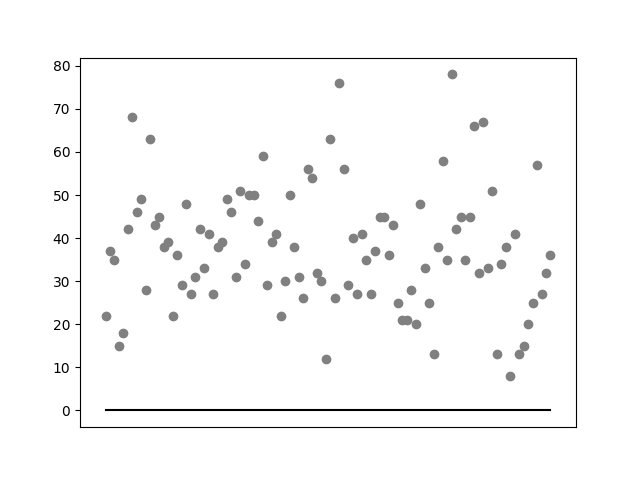
\includegraphics[width=\linewidth]{img/graficos/reta0/alexnet/fig-reta-0-image-treat-1-alexnet-lrelu.png}
	  \end{subfigure}%
	\end{figure}

	Obedecendo ao método de validação cruzada \emph{holdout} previamente mencionado, os resultados desta abordagem encontram-se sintetizados na Tabela \ref{tab:results-1}. É possível constatar que as CNNs com função de ativação \emph{ReLU} obtiveram melhor desempenho, com a arquitetura LeNet, em particular, com resultados ligeiramente superiores.

  \begin{table}[!ht]
		\caption{Resultados do treino e teste dos modelos propostos na Abordagem 1.}
		\label{tab:results-1}
		\begin{center}
			\begin{tabular}{l l l l l}
				\toprule
				Rede & Função de ativação & Épocas & MAE Teste & RMSE Teste \\
				\midrule
				LeNet & \emph{ReLU}  & 4 & 10.53 & 13.55 \\
				LeNet & \emph{Leaky ReLU} & 8 & 38.33 & 40.82 \\
				AlexNet & \emph{ReLU}  & 5 & 11.03 & 13.76 \\
				AlexNet & \emph{Leaky ReLU} & 5 & 39.27 & 41.97 \\
				\bottomrule
			\end{tabular}
		\end{center}
	\end{table}

\section{Abordagem 2: Introduzindo \emph{Data Agumentation}}%com data augmentation, com normalização e sem equalização

	A abordagem anterior consistiu essencialmente da utilização dos modelos tal como foram definidos e com uma simples operação de adequação dos dados de entrada por meio de normalização. Porém, em problemas de Visão Computacional, é comum aplicar técnicas de \emph{data augmentation} com vistas a aumentar artificialmente o conjunto de dados, fazendo com que o modelo, em sua fase de treinamento, não seja exposto à mesma entrada em mais de uma ocasião. Isto previne \emph{overfitting} e colabora para uma melhor generalização \cite{chollet2017deep}.

	As técnicas de \emph{data augmentation} consideradas foram a rotação entre $0$ e $20$ graus no sentido horário ou anti-horário, zoom de $0.8$ a $1.2$ vezes, inversão horizontal com probabilidade de ocorrência de $0.5$ ou translação com probabilidade igual a $0.2$.

	Os gráficos das métricas de desempenho coletadas durante o treinamento e a reta-0 obtida a partir dos dados de teste em cada uma destas quatro configurações são ilustrados nas Figuras \ref{fig:lenet-abordagem2} e \ref{fig:alexnet-abordagem2}.

	\begin{figure}[h!]
		\caption{Resultados do treinamento e teste da CNN LeNet.}\label{fig:lenet-abordagem2}
		\begin{subfigure}[hb]{0.5\linewidth}
			\caption{RMSE de treinamento da arquitetura LeNet utilizando funções de ativação \emph{ReLU}.}
			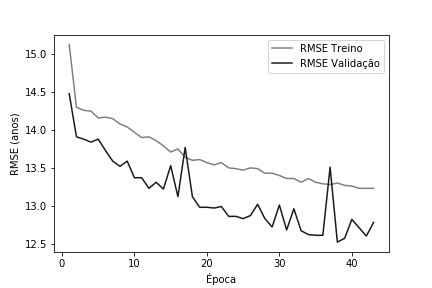
\includegraphics[width=\linewidth]{img/graficos/history/lenet/fig-history-image-treat-2-lenet-relu-rmse.png}%
		\end{subfigure}%
		\begin{subfigure}[hb]{0.5\linewidth}
			\caption{Reta-0 LeNet \emph{ReLU}.}
			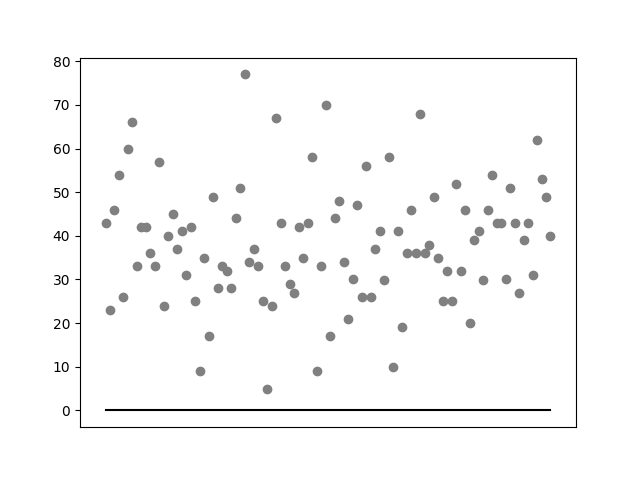
\includegraphics[width=\linewidth]{img/graficos/reta0/lenet/fig-reta-0-image-treat-2-lenet-relu.png}%
		\end{subfigure}\\
		\begin{subfigure}[hb]{0.5\linewidth}
			\caption{RMSE de treinamento da arquitetura LeNet utilizando funções de ativação \emph{Leaky ReLU}.}
			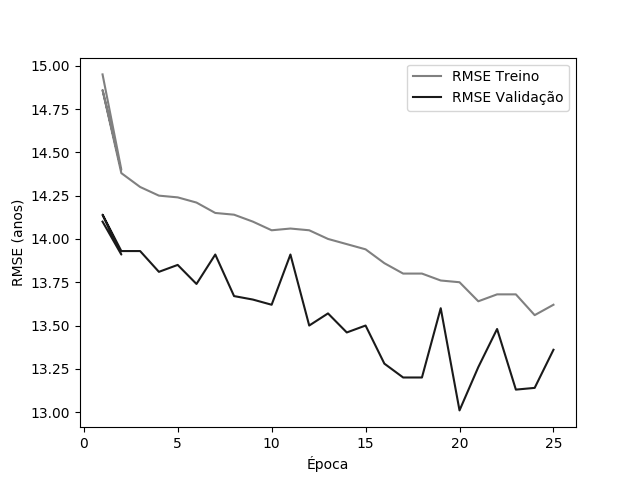
\includegraphics[width=\linewidth]{img/graficos/history/lenet/fig-history-image-treat-2-lenet-lrelu-rmse.png}
		\end{subfigure}
		\begin{subfigure}[hb]{0.5\linewidth}
			\caption{Reta-0 LeNet \emph{Leaky ReLU}.}
		 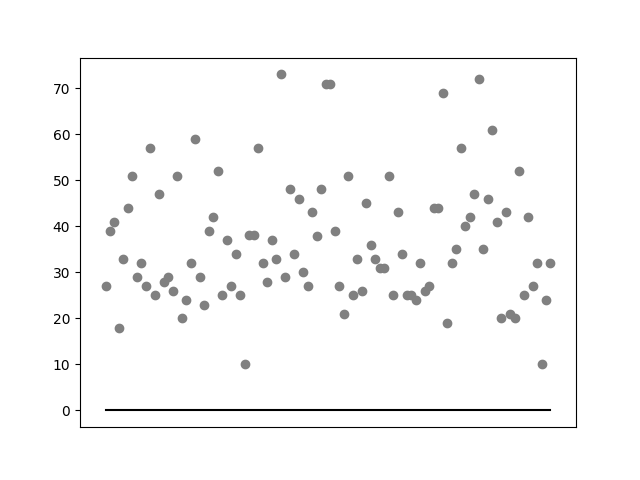
\includegraphics[width=\linewidth]{img/graficos/reta0/lenet/fig-reta-0-image-treat-2-lenet-lrelu.png}
		\end{subfigure}%
	\end{figure}

	\begin{figure}[h!]
		\caption{Resultados do treinamento e teste da CNN AlexNet.}\label{fig:alexnet-abordagem2}
		\begin{subfigure}[hb]{0.5\linewidth}
			\caption{Treinamento AlexNet \emph{ReLU}.}
			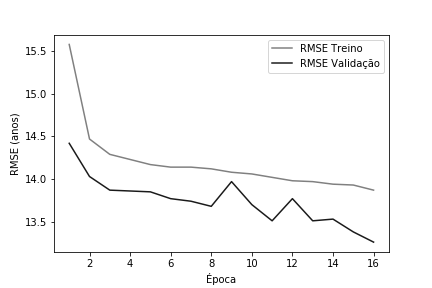
\includegraphics[width=\linewidth]{img/graficos/history/alexnet/fig-history-image-treat-2-alexnet-relu-rmse.png}
		\end{subfigure}
		\begin{subfigure}[hb]{0.5\linewidth}
			\caption{Reta-0 AlexNet \emph{ReLU}.}
			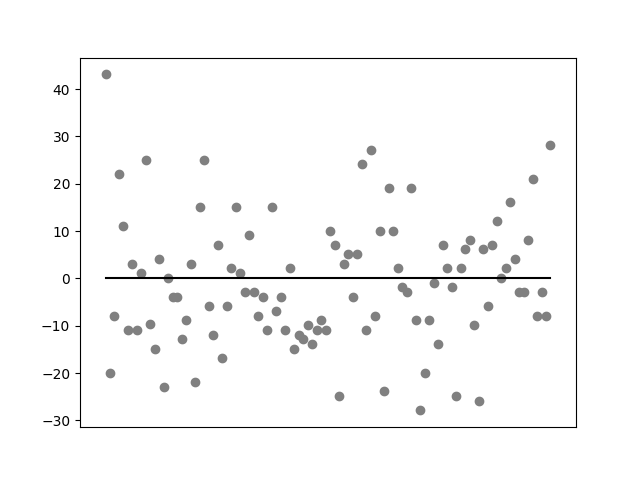
\includegraphics[width=\linewidth]{img/graficos/reta0/alexnet/fig-reta-0-image-treat-2-alexnet-relu.png}%
		\end{subfigure}\\
		\begin{subfigure}[hb]{0.5\linewidth}
			\caption{Treinamento AlexNet \emph{Leaky ReLU}.}
			\centering
			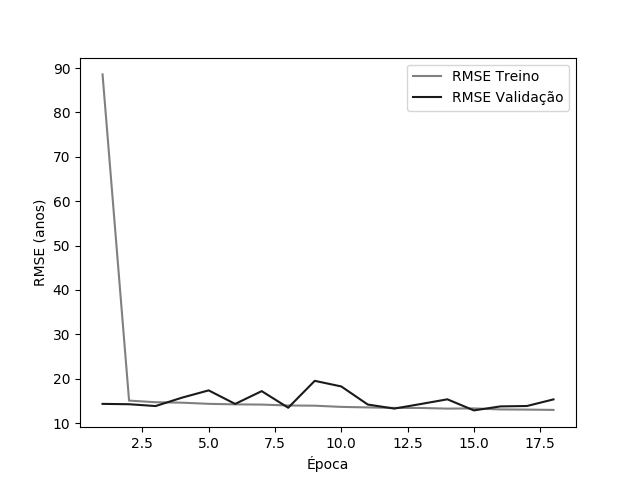
\includegraphics[width=\linewidth]{img/graficos/history/alexnet/fig-history-image-treat-2-alexnet-lrelu-rmse.png}
		\end{subfigure}
		\begin{subfigure}[hb]{0.5\linewidth}
			\caption{Reta-0 AlexNet \emph{Leaky ReLU}.}
			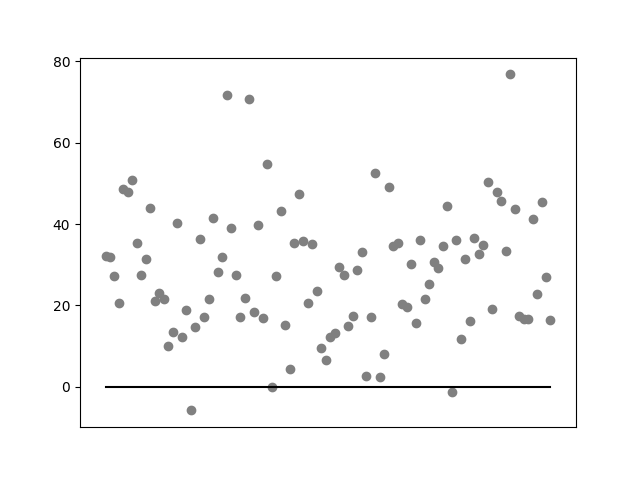
\includegraphics[width=\linewidth]{img/graficos/reta0/alexnet/fig-reta-0-image-treat-2-alexnet-lrelu.png}
		\end{subfigure}%
	\end{figure}

	De maneira análoga, as métricas de desempenho coletadas encontram-se detalhadas na Tabela \ref{tab:results2}. Nota-se que o número de épocas no treinamento foi maior que a abordagem anterior, indicando que houve um cenário mais favorável para o aprendizado dos padrões nos dados. De maneira geral, as métricas obtidas não fornecem uma evidência forte de que esta segunda abordagem produz resultados mais significativos que a primeira mas, no caso da CNN AlexNet com \emph{ReLU}, os resultados foram comparáveis.

	\begin{table}[!ht]
		\caption{Resultados do treino e teste dos modelos propostos na Abordagem 2.}
		\label{tab:results2}
		\begin{center}
			\begin{tabular}{l l l l l}
				\toprule
				Rede & Função de ativação & Épocas & MAE Teste & RMSE Teste \\
				\midrule
				LeNet & \emph{ReLU}  & 39 & 37.85 & 40.27 \\
				LeNet & \emph{Leaky ReLU} & 21 & 38.50 & 41.06 \\
				AlexNet & \emph{ReLU}  & 16 & 11.59 & 14.59 \\
				AlexNet & \emph{Leaky ReLU} & 16 & 28.06 & 31.81 \\
				\bottomrule
			\end{tabular}
		\end{center}
	\end{table}

	O efeito positivo esperado pelo \emph{data augmentation} não se mostrou tão evidente quanto se esperava inicialmente. Porém, isto pode acontecer em razão dos valores dos hiperparâmetros e da necessidade de melhor pré-processamento das imagens antes da apresentação às CNNs, o que motivou a realização da abordagem a seguir.


\section{Abordagem 3: Introduzindo Equalização de Histograma}%com data augmentation, com normalização e com equalização
	A terceira abordagem utilizou as imagens da base de dados normalizadas e com equalização de histograma de cores, além de técnicas de \emph{data augmentation}, que inclui a probabilidade de uma rotação entre 0 e 20 graus, zoom de 0.8 a 1.2, chance de flip de 0.5, translate de 0.2.

	%A CNN que implementa a arquitetura LeNet com função de ativação \emph{ReLU} foi treinada por 43 épocas, obteve MAE de $14.09$ e RMSE $17.93$. A LeNet com função de ativação \emph{Leaky ReLU} foi treinada por 15 épocas, obteve MAE de $14.44$ anos e RMSE de $18.18$ anos. Os treinamentos duraram aproximadamente $16$ e $12$ horas respectivamente, em uma instância do Google Compute Engine com 4 CPus virtuais e 15 GB de RAM. Os gráficos de treinamento e as retas zero obtidas a partir da apresentação do conjunto de teste aos modelos consolidados podem ser vistos na Figura \ref{fig:lenet-abordagem1}. É possível notar que ambas as redes sofreram com \emph{overfitting} e obtiveram grande margem de erro, no entanto a LeNet que utilizou \emph{Leaky ReLU} como função de ativação obteve um desempenho mais satisfatório.

	\begin{figure}[hb!]
		\caption{Resultados do treinamento e teste da CNN LeNet.}\label{fig:lenet-abordagem1}
		\begin{subfigure}[hb]{0.5\linewidth}
			\caption{RMSE de treinamento da arquitetura LeNet utilizando funções de ativação \emph{ReLU}.}
			\label{fig:redeneuralbiologica}
			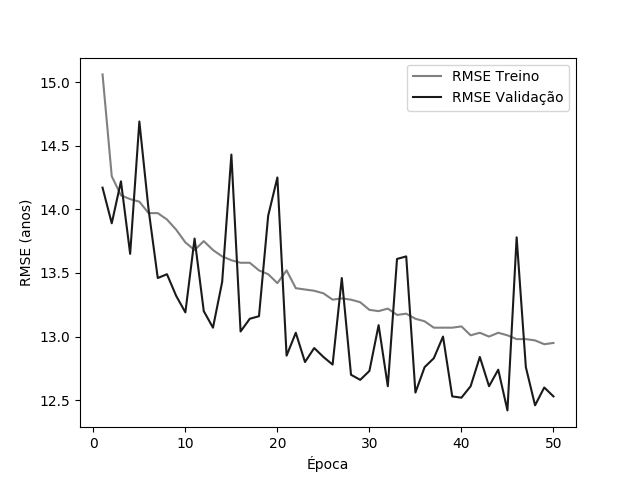
\includegraphics[width=\linewidth]{img/graficos/history/lenet/fig-history-image-treat-3-lenet-relu-rmse.png}%
		\end{subfigure}%
		\begin{subfigure}[hb]{0.5\linewidth}
			\caption{Reta-0 LeNet \emph{ReLU}.}
			\label{fig:redeneuralbiologica}
			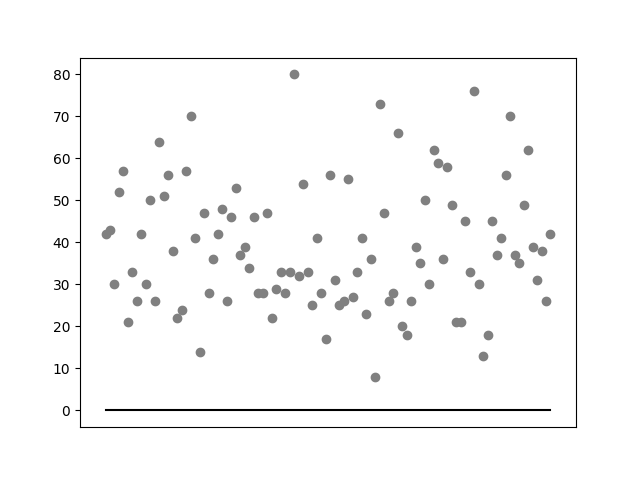
\includegraphics[width=\linewidth]{img/graficos/reta0/lenet/fig-reta-0-image-treat-3-lenet-relu.png}%
		\end{subfigure}\\
		\begin{subfigure}[hb]{0.5\linewidth}
			\caption{RMSE de treinamento da arquitetura LeNet utilizando funções de ativação \emph{Leaky ReLU}.}
			\label{fig:redeneuralbiologica}
			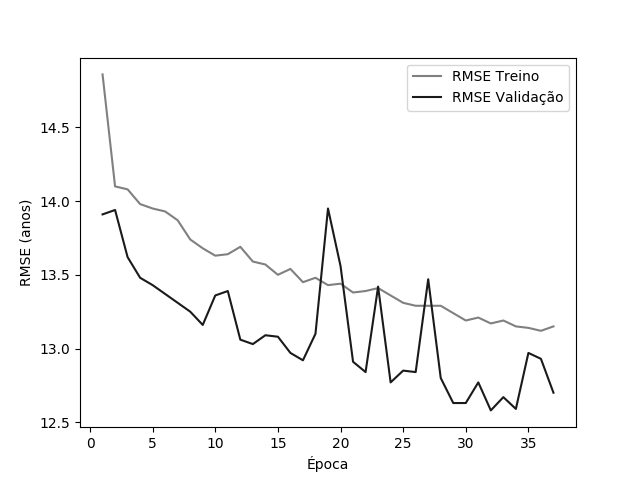
\includegraphics[width=\linewidth]{img/graficos/history/lenet/fig-history-image-treat-3-lenet-lrelu-rmse.png}
		\end{subfigure}
		\begin{subfigure}[hb]{0.5\linewidth}
			\caption{Reta-0 LeNet \emph{Leaky ReLU}.}
			\label{fig:redeneuralbiologica}
		 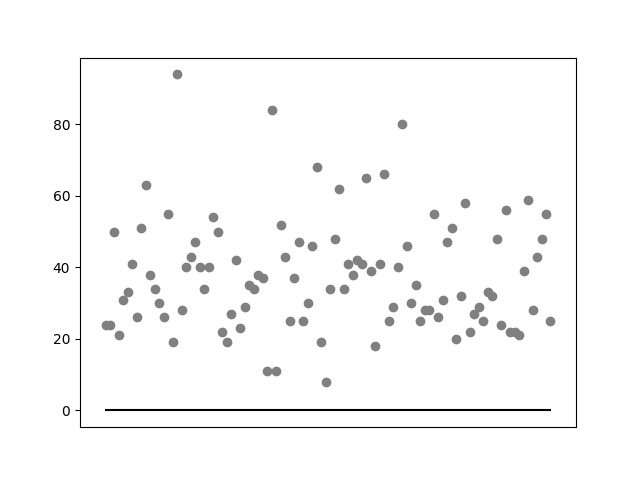
\includegraphics[width=\linewidth]{img/graficos/reta0/lenet/fig-reta-0-image-treat-3-lenet-lrelu.png}
		\end{subfigure}%
	\end{figure}

	%A CNN que implementa a arquitetura AlexNet com função de ativação \emph{ReLU} foi treinada por 10 épocas, obteve MAE de $38.63$ anos e RMSE de $41.22$ anos. A AlexNet com função de ativação \emph{Leaky ReLU} foi treinada por 30 épocas, obteve MAE de $14.44$ anos e RMSE de $15.33$ anos. Os treinamentos duraram aproximadamente $15$ e $38$ horas respectivamente, na mesma instância do Google Compute Engine utilizada para o treinamento das redes LeNet. Os gráficos de treinamento e as retas zero obtidas a partir da apresentação do conjunto de teste aos modelos consolidados podem ser vistos na Figura \ref{fig:alexnet-abordagem1}. É possível notar que a AlexNet que utiliza \emph{ReLU} sofreu de \emph{dying ReLU problem}, o que culminou em previsões iguais a zero para todos os exemplos do conjunto de teste, o que pode ser evidenciado pela ausência total de acertos conforme mostra a Figura \ref{fig:reta0reludying}. Para contornar este problema, a AlexNet que utilizou \emph{Leaky ReLU} como função de ativação foi capaz de convergir para uma solução mais adequada, prevendo idades mais próximas às reais.

	\begin{figure}[hb!]
		\caption{Resultados do treinamento e teste da CNN AlexNet.}\label{fig:alexnet-abordagem1}
		\begin{subfigure}[hb]{0.5\linewidth}
			\caption{Treinamento AlexNet \emph{ReLU}.}
			\label{fig:redeneuralbiologica}
			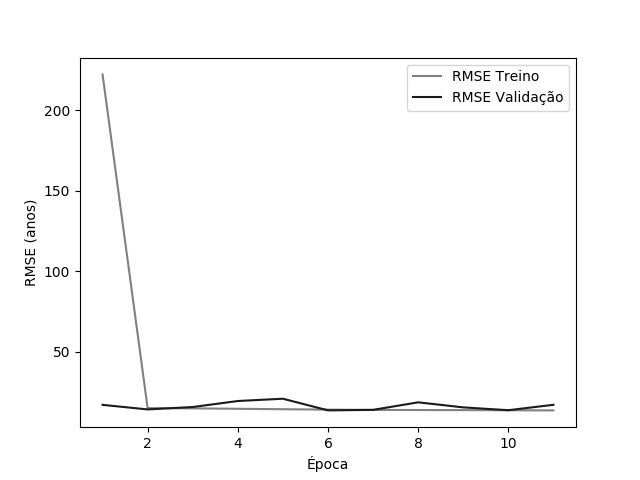
\includegraphics[width=\linewidth]{img/graficos/history/alexnet/fig-history-image-treat-3-alexnet-relu-rmse.png}
		\end{subfigure}
		\begin{subfigure}[hb]{0.5\linewidth}
			\caption{Reta-0 AlexNet \emph{ReLU}.}
			\label{fig:reta0reludying}
			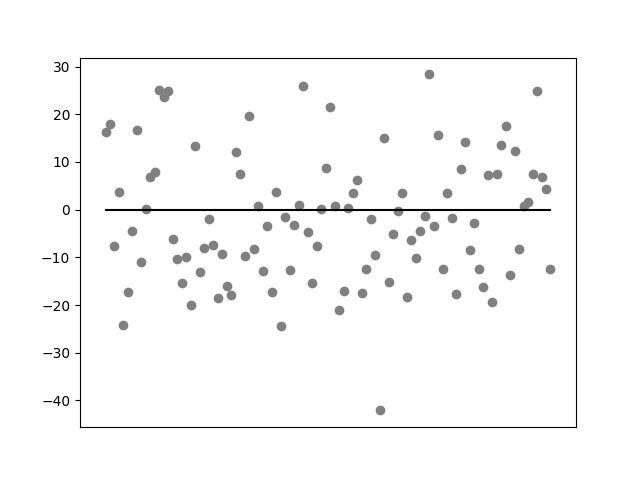
\includegraphics[width=\linewidth]{img/graficos/reta0/alexnet/fig-reta-0-image-treat-3-alexnet-relu.png}%
		\end{subfigure}\\
		\begin{subfigure}[hb]{0.5\linewidth}
			\caption{Treinamento AlexNet \emph{Leaky ReLU}.}
			\label{fig:histalexlrelunorm}
			\centering
			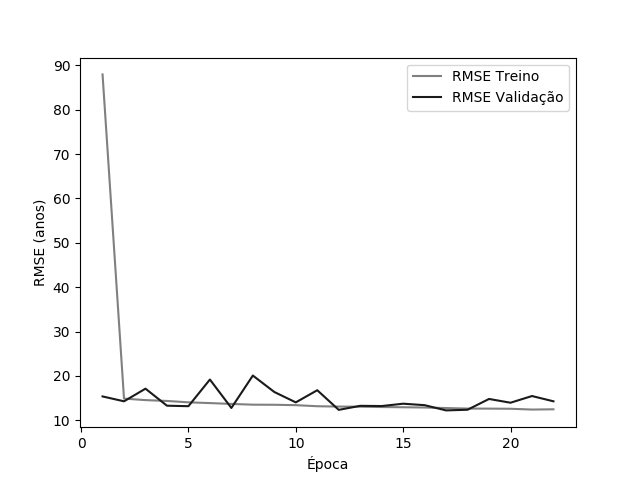
\includegraphics[width=\linewidth]{img/graficos/history/alexnet/fig-history-image-treat-3-alexnet-lrelu-rmse.png}
		\end{subfigure}
		\begin{subfigure}[hb]{0.5\linewidth}
			\caption{Reta-0 AlexNet \emph{Leaky ReLU}.}
			\label{fig:redeneuralbiologica}
			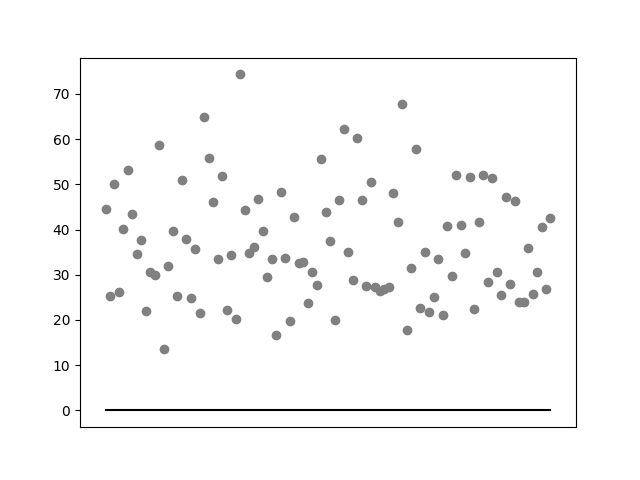
\includegraphics[width=\linewidth]{img/graficos/reta0/alexnet/fig-reta-0-image-treat-3-alexnet-lrelu.png}
		\end{subfigure}%
	\end{figure}


	% \begin{figure}[hb!]
	% 	\caption{LEGENDA.}
	% 	\begin{subfigure}[hb]{0.5\linewidth}
	% 		\caption{Reta-0 Alexnet LRelU com imagens normalizadas e equalizadas}
	% 		\label{fig:histalexlrelunorm}
	% 		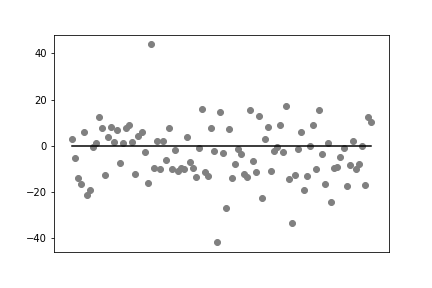
\includegraphics[width=\linewidth]{img/graficos/fig-reta-0-alexnet-lrelu-data-augmentation-2-2.png}
	% 	\end{subfigure}%
	% 	\begin{subfigure}[hb]{0.5\linewidth}
	% 		\caption{Reta-0 Alexnet ReLU com imagens normalizadas e equalizadas}
	% 		\label{fig:redeneuralbiologica}
	% 		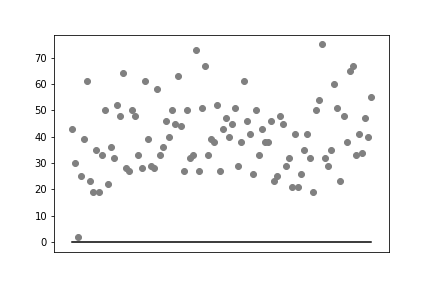
\includegraphics[width=\linewidth]{img/graficos/fig-reta-0-alexnet-relu-data-augmentation-2-1.png}
	% 	\end{subfigure}
	% \end{figure}

	Obedecendo ao método de validação cruzada \emph{holdout} previamente mencionado, os resultados desta abordagem encontram-se sintetizados na Tabela \ref{tab:results-2}.

	\begin{table}[!ht]
		\caption{Resultados do treino e teste dos modelos propostos na Abordagem 1.}
		\label{tab:results-2}
		\begin{adjustbox}{width=1\textwidth}
			\begin{tabular}{l l l l l l l}
				\toprule
				Rede & Função de ativação & Parâmetros & Épocas & Tempo de treinamento & MAE Teste & RMSE Teste \\
				\midrule
				LeNet & \emph{Leaky ReLU} & params & 15 & 12 h & 14.44 & 18.18 \\
				LeNet & \emph{ReLU} & params & 43 & 16 h & 14.09 & 17.93 \\
				AlexNet & \emph{ReLU} & $58.286.145$ & 10 & 15 h & 38.63 & 41.22 \\
				AlexNet & \emph{Leaky ReLU} & params & 30 & 40 h & 15.33 & 18.58 \\
				\bottomrule
			\end{tabular}
		\end{adjustbox}
	\end{table}

\section{Abordagem 4}%com data augmentation, com normalização e com equalização, usando mae pra loss
	A quarta abordagem utilizou as imagens da base de dados normalizadas e com equalização de histograma de cores, além de técnicas de \emph{data augmentation}, que inclui a probabilidade de uma rotação entre 0 e 20 graus, zoom de 0.8 a 1.2, chance de flip de 0.5, translate de 0.2. Porém, utilizou-se a métrica MAE para o cálculo da atualização dos pesos (como loss). Neste ponto, escolheu-se a \todo{criterio} dentre as treinadas nas abordagens anteriores, ou seja, a rede LeNet com função de ativaçao Relu.

	%A CNN que implementa a arquitetura LeNet com função de ativação \emph{ReLU} foi treinada por 43 épocas, obteve MAE de $14.09$ e RMSE $17.93$. A LeNet com função de ativação \emph{Leaky ReLU} foi treinada por 15 épocas, obteve MAE de $14.44$ anos e RMSE de $18.18$ anos. Os treinamentos duraram aproximadamente $16$ e $12$ horas respectivamente, em uma instância do Google Compute Engine com 4 CPus virtuais e 15 GB de RAM. Os gráficos de treinamento e as retas zero obtidas a partir da apresentação do conjunto de teste aos modelos consolidados podem ser vistos na Figura \ref{fig:lenet-abordagem1}. É possível notar que ambas as redes sofreram com \emph{overfitting} e obtiveram grande margem de erro, no entanto a LeNet que utilizou \emph{Leaky ReLU} como função de ativação obteve um desempenho mais satisfatório.

	\begin{figure}[hb!]
		\caption{Resultados do treinamento e teste da CNN LeNet.}\label{fig:lenet-abordagem1}
		\begin{subfigure}[hb]{0.5\linewidth}
			\caption{RMSE de treinamento da arquitetura LeNet utilizando funções de ativação \emph{ReLU}.}
			\label{fig:redeneuralbiologica}
			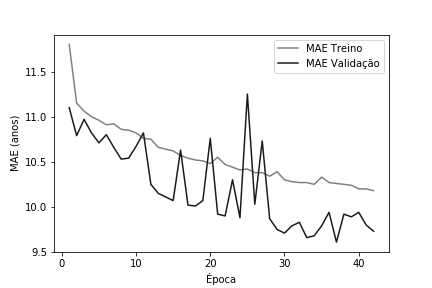
\includegraphics[width=\linewidth]{img/graficos/history/lenet/fig-history-abordagem-4-lenet-relu-mae.png}%
		\end{subfigure}%
		\begin{subfigure}[hb]{0.5\linewidth}
			\caption{Reta-0 LeNet \emph{ReLU}.}
			\label{fig:redeneuralbiologica}
			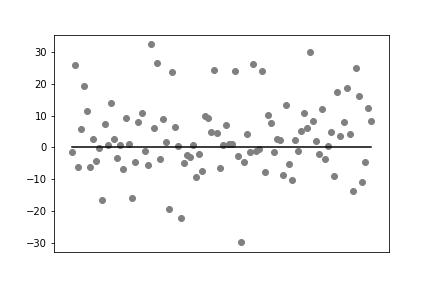
\includegraphics[width=\linewidth]{img/graficos/reta0/lenet/fig-reta-0-abordagem-4-lenet-relu.png}%
		\end{subfigure}\\
	\end{figure}

	%A CNN que implementa a arquitetura AlexNet com função de ativação \emph{ReLU} foi treinada por 10 épocas, obteve MAE de $38.63$ anos e RMSE de $41.22$ anos. A AlexNet com função de ativação \emph{Leaky ReLU} foi treinada por 30 épocas, obteve MAE de $14.44$ anos e RMSE de $15.33$ anos. Os treinamentos duraram aproximadamente $15$ e $38$ horas respectivamente, na mesma instância do Google Compute Engine utilizada para o treinamento das redes LeNet. Os gráficos de treinamento e as retas zero obtidas a partir da apresentação do conjunto de teste aos modelos consolidados podem ser vistos na Figura \ref{fig:alexnet-abordagem1}. É possível notar que a AlexNet que utiliza \emph{ReLU} sofreu de \emph{dying ReLU problem}, o que culminou em previsões iguais a zero para todos os exemplos do conjunto de teste, o que pode ser evidenciado pela ausência total de acertos conforme mostra a Figura \ref{fig:reta0reludying}. Para contornar este problema, a AlexNet que utilizou \emph{Leaky ReLU} como função de ativação foi capaz de convergir para uma solução mais adequada, prevendo idades mais próximas às reais.

	% \begin{figure}[hb!]
	% 	\caption{LEGENDA.}
	% 	\begin{subfigure}[hb]{0.5\linewidth}
	% 		\caption{Reta-0 Alexnet LRelU com imagens normalizadas e equalizadas}
	% 		\label{fig:histalexlrelunorm}
	% 		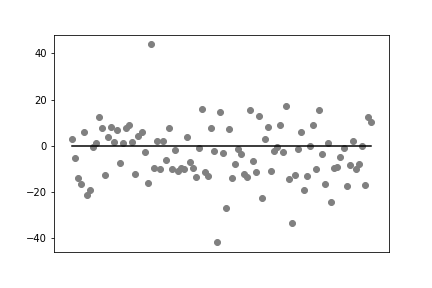
\includegraphics[width=\linewidth]{img/graficos/fig-reta-0-alexnet-lrelu-data-augmentation-2-2.png}
	% 	\end{subfigure}%
	% 	\begin{subfigure}[hb]{0.5\linewidth}
	% 		\caption{Reta-0 Alexnet ReLU com imagens normalizadas e equalizadas}
	% 		\label{fig:redeneuralbiologica}
	% 		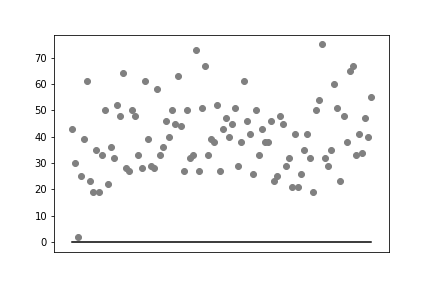
\includegraphics[width=\linewidth]{img/graficos/fig-reta-0-alexnet-relu-data-augmentation-2-1.png}
	% 	\end{subfigure}
	% \end{figure}

	Obedecendo ao método de validação cruzada \emph{holdout} previamente mencionado, os resultados desta abordagem encontram-se sintetizados na Tabela \ref{tab:results-2}.

	\begin{table}[!ht]
		\caption{Resultados do treino e teste dos modelos propostos na Abordagem 1.}
		\label{tab:results-2}
		\begin{adjustbox}{width=1\textwidth}
			\begin{tabular}{l l l l l l l}
				\toprule
				Rede & Função de ativação & Parâmetros & Épocas & Tempo de treinamento & MAE Teste & RMSE Teste \\
				\midrule
				LeNet & \emph{Leaky ReLU} & params & 15 & 12 h & 14.44 & 18.18 \\
				LeNet & \emph{ReLU} & params & 43 & 16 h & 14.09 & 17.93 \\
				AlexNet & \emph{ReLU} & $58.286.145$ & 10 & 15 h & 38.63 & 41.22 \\
				AlexNet & \emph{Leaky ReLU} & params & 30 & 40 h & 15.33 & 18.58 \\
				\bottomrule
			\end{tabular}
		\end{adjustbox}
	\end{table}


\section{Abordagem 5}% sem data augmentation, com normalização e sem equalização, usando mae pra loss, batch de 128, sem patience
	A quinta abordagem utilizou as imagens da base de dados normalizadas, mas sem equalização de histograma de cores, e técnicas de \emph{data augmentation}. Porém, seguiu-se utilizando a métrica MAE para o cálculo da atualização dos pesos (como loss), e aumentou-se o tamanho do batch para 128, haja vista a característica instável do treinamento mostrada nas abordagens anteriores. Utilizou-se somente da arquitetura LeNet ReLU sem histograma e data augmentation por ser a que alcançou menor RMSE dentre as treinadas nas abordagens anteriores.

	%A CNN que implementa a arquitetura LeNet com função de ativação \emph{ReLU} foi treinada por 43 épocas, obteve MAE de $14.09$ e RMSE $17.93$. A LeNet com função de ativação \emph{Leaky ReLU} foi treinada por 15 épocas, obteve MAE de $14.44$ anos e RMSE de $18.18$ anos. Os treinamentos duraram aproximadamente $16$ e $12$ horas respectivamente, em uma instância do Google Compute Engine com 4 CPus virtuais e 15 GB de RAM. Os gráficos de treinamento e as retas zero obtidas a partir da apresentação do conjunto de teste aos modelos consolidados podem ser vistos na Figura \ref{fig:lenet-abordagem1}. É possível notar que ambas as redes sofreram com \emph{overfitting} e obtiveram grande margem de erro, no entanto a LeNet que utilizou \emph{Leaky ReLU} como função de ativação obteve um desempenho mais satisfatório.

	\begin{figure}[hb!]
		\caption{Resultados do treinamento e teste da CNN LeNet.}\label{fig:lenet-abordagem1}
		\begin{subfigure}[hb]{0.5\linewidth}
			\caption{RMSE de treinamento da arquitetura LeNet utilizando funções de ativação \emph{ReLU}.}
			\label{fig:redeneuralbiologica}
			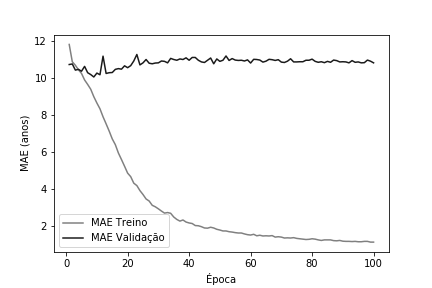
\includegraphics[width=\linewidth]{img/graficos/history/lenet/fig-history-abordagem-5-lenet-relu-mae.png}%
		\end{subfigure}%
		\begin{subfigure}[hb]{0.5\linewidth}
			\caption{Reta-0 LeNet \emph{ReLU}.}
			\label{fig:redeneuralbiologica}
			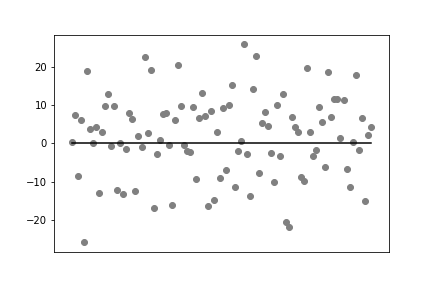
\includegraphics[width=\linewidth]{img/graficos/reta0/lenet/fig-reta-0-abordagem-5-lenet-relu.png}%
		\end{subfigure}\\
	\end{figure}

	%A CNN que implementa a arquitetura AlexNet com função de ativação \emph{ReLU} foi treinada por 10 épocas, obteve MAE de $38.63$ anos e RMSE de $41.22$ anos. A AlexNet com função de ativação \emph{Leaky ReLU} foi treinada por 30 épocas, obteve MAE de $14.44$ anos e RMSE de $15.33$ anos. Os treinamentos duraram aproximadamente $15$ e $38$ horas respectivamente, na mesma instância do Google Compute Engine utilizada para o treinamento das redes LeNet. Os gráficos de treinamento e as retas zero obtidas a partir da apresentação do conjunto de teste aos modelos consolidados podem ser vistos na Figura \ref{fig:alexnet-abordagem1}. É possível notar que a AlexNet que utiliza \emph{ReLU} sofreu de \emph{dying ReLU problem}, o que culminou em previsões iguais a zero para todos os exemplos do conjunto de teste, o que pode ser evidenciado pela ausência total de acertos conforme mostra a Figura \ref{fig:reta0reludying}. Para contornar este problema, a AlexNet que utilizou \emph{Leaky ReLU} como função de ativação foi capaz de convergir para uma solução mais adequada, prevendo idades mais próximas às reais.

	% \begin{figure}[hb!]
	% 	\caption{LEGENDA.}
	% 	\begin{subfigure}[hb]{0.5\linewidth}
	% 		\caption{Reta-0 Alexnet LRelU com imagens normalizadas e equalizadas}
	% 		\label{fig:histalexlrelunorm}
	% 		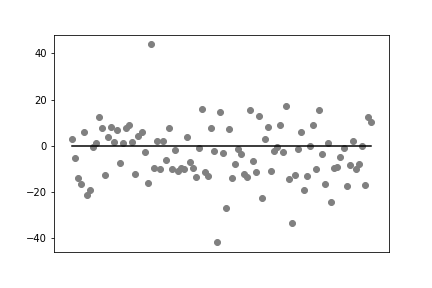
\includegraphics[width=\linewidth]{img/graficos/fig-reta-0-alexnet-lrelu-data-augmentation-2-2.png}
	% 	\end{subfigure}%
	% 	\begin{subfigure}[hb]{0.5\linewidth}
	% 		\caption{Reta-0 Alexnet ReLU com imagens normalizadas e equalizadas}
	% 		\label{fig:redeneuralbiologica}
	% 		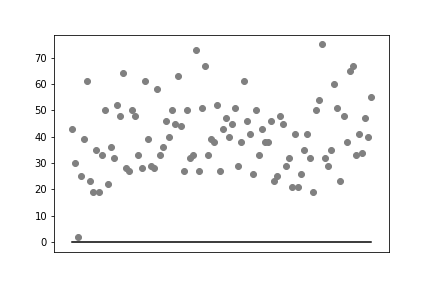
\includegraphics[width=\linewidth]{img/graficos/fig-reta-0-alexnet-relu-data-augmentation-2-1.png}
	% 	\end{subfigure}
	% \end{figure}

	Obedecendo ao método de validação cruzada \emph{holdout} previamente mencionado, os resultados desta abordagem encontram-se sintetizados na Tabela \ref{tab:results-2}.

	\begin{table}[!ht]
		\caption{Resultados do treino e teste dos modelos propostos na Abordagem 1.}
		\label{tab:results-2}
		\begin{adjustbox}{width=1\textwidth}
			\begin{tabular}{l l l l l l l}
				\toprule
				Rede & Função de ativação & Parâmetros & Épocas & Tempo de treinamento & MAE Teste & RMSE Teste \\
				\midrule
				LeNet & \emph{Leaky ReLU} & params & 15 & 12 h & 14.44 & 18.18 \\
				LeNet & \emph{ReLU} & params & 43 & 16 h & 14.09 & 17.93 \\
				AlexNet & \emph{ReLU} & $58.286.145$ & 10 & 15 h & 38.63 & 41.22 \\
				AlexNet & \emph{Leaky ReLU} & params & 30 & 40 h & 15.33 & 18.58 \\
				\bottomrule
			\end{tabular}
		\end{adjustbox}
	\end{table}



% \section{Abordagem 1}%fase2
% A primeira abordagem de treinamento das CNNs utilizou as imagens da base de dados com equalização por histograma de frequência, normalizadas, e com $50\%$ de chance de estarem rotacionadas horizontalmente. Conforme mencionado na Seção \ref{subsec:modelos}, os treinamentos e testes compreenderam as arquiteturas canônicas LeNet e AlexNet com funções de ativação \emph{ReLU} e \emph{Leaky ReLU} nas camadas ocultas e de ativação. É importante ressaltar que neste momento não foram utilizadas técnicas de \emph{transfer learning}.
%
% % Explicação da le net, gráficos da le net
% A CNN que implementa a arquitetura LeNet com função de ativação \emph{ReLU} foi treinada por 43 épocas, obteve MAE de $14.09$ e RMSE $17.93$. A LeNet com função de ativação \emph{Leaky ReLU} foi treinada por 15 épocas, obteve MAE de $14.44$ anos e RMSE de $18.18$ anos. Os treinamentos duraram aproximadamente $16$ e $12$ horas respectivamente, em uma instância do Google Compute Engine com 4 CPus virtuais e 15 GB de RAM. Os gráficos de treinamento e as retas zero obtidas a partir da apresentação do conjunto de teste aos modelos consolidados podem ser vistos na Figura \ref{fig:lenet-abordagem1}. É possível notar que ambas as redes sofreram com \emph{overfitting} e obtiveram grande margem de erro, no entanto a LeNet que utilizou \emph{Leaky ReLU} como função de ativação obteve um desempenho mais satisfatório.
%
% \begin{figure}[hb!]
% 	\caption{Resultados do treinamento e teste da CNN LeNet.}\label{fig:lenet-abordagem1}
%   \begin{subfigure}[hb]{0.5\linewidth}
%     \caption{RMSE de treinamento da arquitetura LeNet utilizando funções de ativação \emph{ReLU}.}
%     \label{fig:redeneuralbiologica}
%     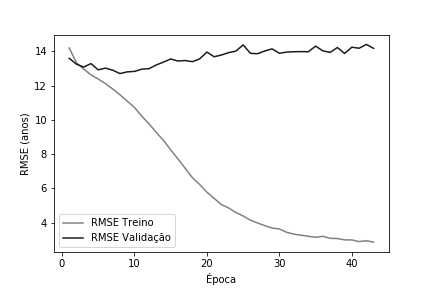
\includegraphics[width=\linewidth]{img/graficos/fig-history-lenet-relu-data-augmentation-2-1.png}%
%   \end{subfigure}%
% 	\begin{subfigure}[hb]{0.5\linewidth}
% 		\caption{Reta-0 LeNet \emph{ReLU}.}
% 		\label{fig:redeneuralbiologica}
% 		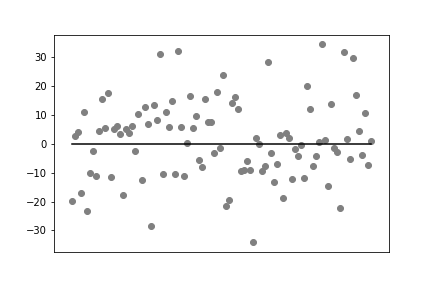
\includegraphics[width=\linewidth]{img/graficos/fig-reta-0-lenetregressor-relu-data-augmentation-2-1.png}%
% 	\end{subfigure}\\
%   \begin{subfigure}[hb]{0.5\linewidth}
%     \caption{RMSE de treinamento da arquitetura LeNet utilizando funções de ativação \emph{Leaky ReLU}.}
%     \label{fig:redeneuralbiologica}
%     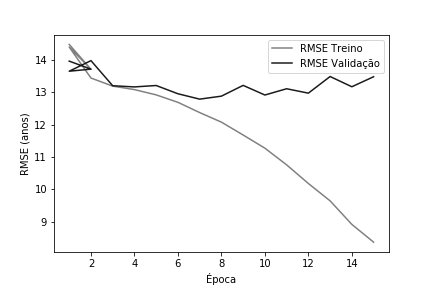
\includegraphics[width=\linewidth]{img/graficos/fig-history-lenet-lrelu-data-augmentation-2-2.png}
%   \end{subfigure}
% 	\begin{subfigure}[hb]{0.5\linewidth}
% 		\caption{Reta-0 LeNet \emph{Leaky ReLU}.}
% 		\label{fig:redeneuralbiologica}
% 	 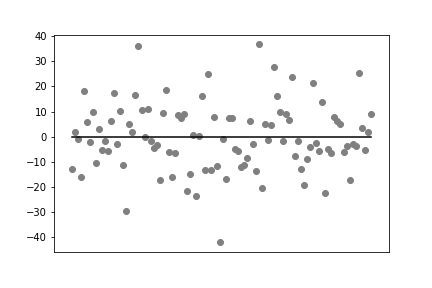
\includegraphics[width=\linewidth]{img/graficos/fig-reta-0-lenetregressor-lrelu-data-augmentation-2-2.png}
% 	\end{subfigure}%
% \end{figure}
%
% A CNN que implementa a arquitetura AlexNet com função de ativação \emph{ReLU} foi treinada por 10 épocas, obteve MAE de $38.63$ anos e RMSE de $41.22$ anos. A AlexNet com função de ativação \emph{Leaky ReLU} foi treinada por 30 épocas, obteve MAE de $14.44$ anos e RMSE de $15.33$ anos. Os treinamentos duraram aproximadamente $15$ e $38$ horas respectivamente, na mesma instância do Google Compute Engine utilizada para o treinamento das redes LeNet. Os gráficos de treinamento e as retas zero obtidas a partir da apresentação do conjunto de teste aos modelos consolidados podem ser vistos na Figura \ref{fig:alexnet-abordagem1}. É possível notar que a AlexNet que utiliza \emph{ReLU} sofreu de \emph{dying ReLU problem}, o que culminou em previsões iguais a zero para todos os exemplos do conjunto de teste, o que pode ser evidenciado pela ausência total de acertos conforme mostra a Figura \ref{fig:reta0reludying}. Para contornar este problema, a AlexNet que utilizou \emph{Leaky ReLU} como função de ativação foi capaz de convergir para uma solução mais adequada, prevendo idades mais próximas às reais.
%
% \begin{figure}[hb!]
% 	\caption{Resultados do treinamento e teste da CNN AlexNet.}\label{fig:alexnet-abordagem1}
% 	\begin{subfigure}[hb]{0.5\linewidth}
% 		\caption{Treinamento AlexNet \emph{ReLU}.}
% 		\label{fig:redeneuralbiologica}
% 		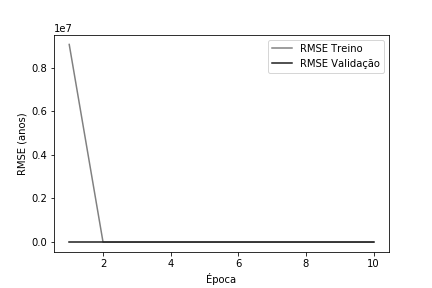
\includegraphics[width=\linewidth]{img/graficos/fig-history-alexnet-relu-data-augmentation-2-1.png}
% 	\end{subfigure}
%   \begin{subfigure}[hb]{0.5\linewidth}
%     \caption{Reta-0 AlexNet \emph{ReLU}.}
%     \label{fig:reta0reludying}
%     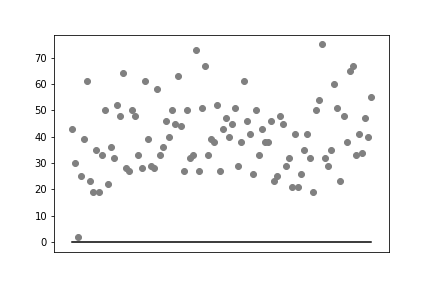
\includegraphics[width=\linewidth]{img/graficos/fig-reta-0-alexnet-relu-data-augmentation-2-1.png}%
%   \end{subfigure}\\
% 	\begin{subfigure}[hb]{0.5\linewidth}
% 		\caption{Treinamento AlexNet \emph{Leaky ReLU}.}
% 		\label{fig:histalexlrelunorm}
%     \centering
% 		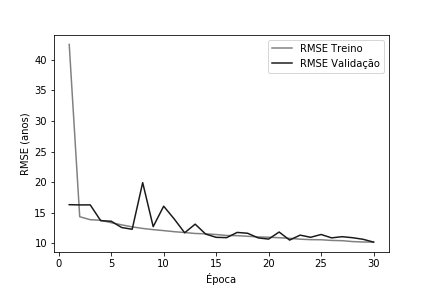
\includegraphics[width=\linewidth]{img/graficos/fig-history-alexnet-lrelu-data-augmentation-2-2.png}
% 	\end{subfigure}
%   \begin{subfigure}[hb]{0.5\linewidth}
%     \caption{Reta-0 AlexNet \emph{Leaky ReLU}.}
%     \label{fig:redeneuralbiologica}
%     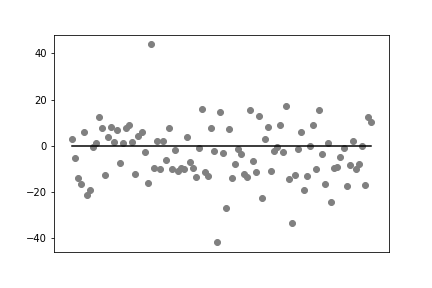
\includegraphics[width=\linewidth]{img/graficos/fig-reta-0-alexnet-lrelu-data-augmentation-2-2.png}
%   \end{subfigure}%
% \end{figure}
%
%
% \begin{figure}[hb!]
% 	\caption{Redes neurais biológicas.}
% 	\begin{subfigure}[hb]{0.5\linewidth}
% 		\caption{Reta-0 Alexnet LRelU com imagens normalizadas e equalizadas}
% 		\label{fig:histalexlrelunorm}
% 		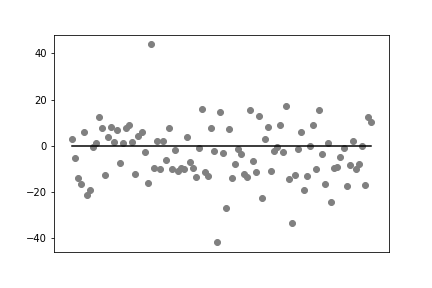
\includegraphics[width=\linewidth]{img/graficos/fig-reta-0-alexnet-lrelu-data-augmentation-2-2.png}
% 	\end{subfigure}%
% 	\begin{subfigure}[hb]{0.5\linewidth}
% 		\caption{Reta-0 Alexnet ReLU com imagens normalizadas e equalizadas}
% 		\label{fig:redeneuralbiologica}
% 		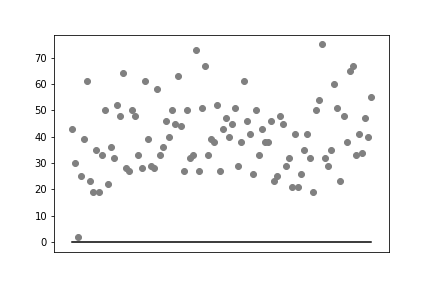
\includegraphics[width=\linewidth]{img/graficos/fig-reta-0-alexnet-relu-data-augmentation-2-1.png}
% 	\end{subfigure}
% \end{figure}
%
% Obedecendo ao método de validação cruzada \emph{holdout} previamente mencionado, os resultados desta abordagem encontram-se sintetizados na Tabela \ref{tab:results-2}.
%
% \begin{table}[!ht]
% 	\caption{Resultados do treino e teste dos modelos propostos na Abordagem 1.}
% 	\label{tab:results-2}
% 	\begin{adjustbox}{width=1\textwidth}
% 		\begin{tabular}{l l l l l l l}
% 			\toprule
% 			Rede & Função de ativação & Parâmetros & Épocas & Tempo de treinamento & MAE Teste & RMSE Teste \\
% 			\midrule
% 			LeNet & \emph{Leaky ReLU} & params & 15 & 12 h & 14.44 & 18.18 \\
% 			LeNet & \emph{ReLU} & params & 43 & 16 h & 14.09 & 17.93 \\
% 			AlexNet & \emph{ReLU} & $58.286.145$ & 10 & 15 h & 38.63 & 41.22 \\
% 			AlexNet & \emph{Leaky ReLU} & params & 30 & 40 h & 15.33 & 18.58 \\
% 			\bottomrule
% 		\end{tabular}
% 	\end{adjustbox}
% \end{table}

\section{Abordagem x}

- Mesmas redes
- Normalização das imagens, equalização por histograma -> o que é
- data augmentation ->  mais técnicas de data augmentation

\section{Abordagem x+1}

Outras arquiteturas
VGG
com transfer learning
1. Retirar última camada (softmax) e adicionar leaky relu
2. Retirar duas últimas camadas (dense e softmax) e adicionar leaky relu
